\documentclass[border=8pt]{standalone}
\usepackage[utf8]{inputenc}
\usepackage{tikz}
\tikzset{
  entita/.style = {rectangle, draw, thick, fill=blue!8, minimum width=28mm, minimum height=16mm, font=\small},
  attr/.style   = {circle, draw, thick, fill=white, minimum size=5pt, inner sep=0},
  pk/.style     = {circle, draw, thick, fill=black, minimum size=5pt, inner sep=0},
  link/.style   = {thick}, et/.style = {font=\footnotesize}
}
\begin{document}
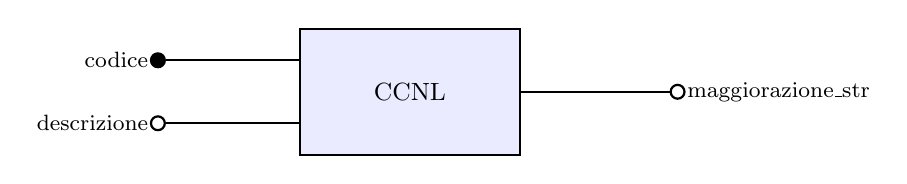
\begin{tikzpicture}
  \node[entita] (E) {CCNL};
  \node[pk]   (c) at (-3.2, 0.4){}; \draw[link] (-1.4, 0.4)--(c); \node[et,left] at (c) {codice};
  \node[attr] (d) at (-3.2,-0.4){}; \draw[link] (-1.4,-0.4)--(d); \node[et,left] at (d) {descrizione};
  \node[attr] (m) at ( 3.4, 0.0){}; \draw[link] ( 1.4, 0.0)--(m); \node[et,right] at (m) {maggiorazione\_str};
\end{tikzpicture}
\end{document}
